% !TEX TS-program = pdflatex
% !TEX encoding = UTF-8 Unicode

% This is a simple template for a LaTeX document using the "article" class.
% See "book", "report", "letter" for other types of document.

\documentclass[11pt]{article} % use larger type; default would be 10pt

\usepackage[utf8]{inputenc} % set input encoding (not needed with XeLaTeX)

%%% Examples of Article customizations
% These packages are optional, depending whether you want the features they provide.
% See the LaTeX Companion or other references for full information.

%%% PAGE DIMENSIONS
\usepackage{geometry} % to change the page dimensions
\geometry{a4paper} % or letterpaper (US) or a5paper or....
% \geometry{margin=2in} % for example, change the margins to 2 inches all round
% \geometry{landscape} % set up the page for landscape
%   read geometry.pdf for detailed page layout information

\usepackage{graphicx} % support the \includegraphics command and options

% \usepackage[parfill]{parskip} % Activate to begin paragraphs with an empty line rather than an indent

%%% PACKAGES
\usepackage{booktabs} % for much better looking tables
\usepackage{array} % for better arrays (eg matrices) in maths
\usepackage{paralist} % very flexible & customisable lists (eg. enumerate/itemize, etc.)
\usepackage{verbatim} % adds environment for commenting out blocks of text & for better verbatim
\usepackage{subfig} % make it possible to include more than one captioned figure/table in a single float
% These packages are all incorporated in the memoir class to one degree or another...

%%% HEADERS & FOOTERS
\usepackage{fancyhdr} % This should be set AFTER setting up the page geometry
\pagestyle{fancy} % options: empty , plain , fancy
\renewcommand{\headrulewidth}{0pt} % customise the layout...
\lhead{}\chead{}\rhead{}
\lfoot{}\cfoot{\thepage}\rfoot{}

%%% SECTION TITLE APPEARANCE
\usepackage{sectsty}
\allsectionsfont{\sffamily\mdseries\upshape} % (See the fntguide.pdf for font help)
% (This matches ConTeXt defaults)

%%% ToC (table of contents) APPEARANCE
\usepackage[nottoc,notlof,notlot]{tocbibind} % Put the bibliography in the ToC
\usepackage[titles,subfigure]{tocloft} % Alter the style of the Table of Contents
\renewcommand{\cftsecfont}{\rmfamily\mdseries\upshape}
\renewcommand{\cftsecpagefont}{\rmfamily\mdseries\upshape} % No bold!

%%% END Article customizations

%%% The "real" document content comes below...

\title{EP06 - Morfologia Matemática \\ Segmentação de placas de carros}
\author{Igor dos Santos Montagner}
%\date{} % Activate to display a given date or no date (if empty),
         % otherwise the current date is printed 

\begin{document}
\maketitle

\section{Requisitos}

O trabalho foi feito em Python utilizando OpenCV 2.3.1. Como esta versão possui uma interface nova em Python incompatível com a anterior, a versão mínima exigida é a 2.3. Para rodar o programa utilize:

 \$ $> $ python license\_plates.py caminho\_para\_imagem

\section{Implementação}

A implementação feita é baseada na determinação de bons marcadores para uma segmentação que utilize o algoritmo Watershed. Deste modo, o procedimento descrito nas próximas subseções visa encontrar um bom marcador para a placa dos carros. 

\subsection{Pré-processamento}

Toda imagem a ser processada é convertida para níveis de cinza e tamanho 640$\times$480. Esta modificação visa normalizar as imagens e facilitar a determinação de tamanhos dos elementos estruturantes utilizados.

\subsection{Determinação do marcador para a placa dos carros}

A determinação do marcador é feita em 8 passos e é baseada no realce dos dígitos escritos na placa do carro. 
\newpage

\subsubsection{Passo 1 - Realce dos dígitos da placa}
	Esta etapa consiste na realização de uma operação \emph{Black Top Hat} com elemento estruturante $7\times7$ na imagem original em níveis de cinza. Esta operação realça os dígitos da placa melhor que a operação de gradiente, pois além de manter os dígitos elimina algumas partes da imagem. O resultado pode ser visto na figura~\ref{step0}.
	\begin{figure}[!h]
		\begin{center}
		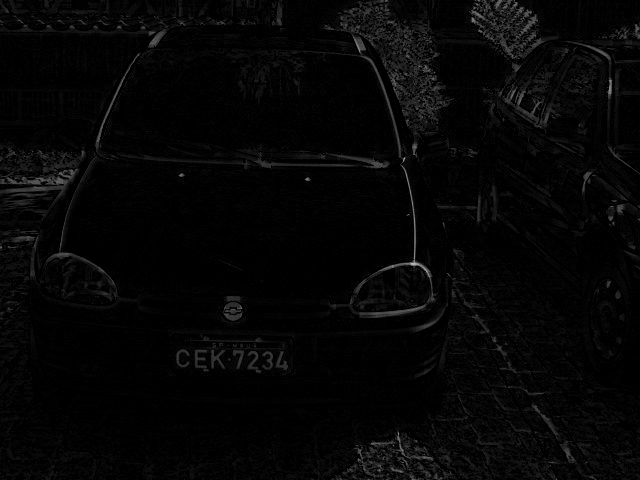
\includegraphics[scale=0.5]{img_relatorio/step0.png}
		\caption{Passo 1 - Realce dos dígitos da placa}\label{step0}
		\end{center}
	\end{figure}
\newpage

\subsubsection{Passo 2 - Limiarização da imagem}
	A imagem é limiarizada utilizando $t = 30$. Como os dígitos são mantidos com nível de cinza relativamente alto pela operação anterior, eles não são eliminados pela limiarização. O resultado pode ser visto na figura~\ref{step0}.
	\begin{figure}[!h]
		\begin{center}
		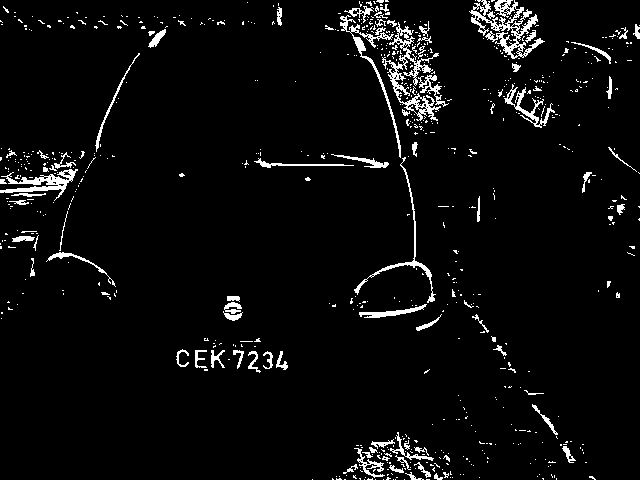
\includegraphics[scale=0.5]{img_relatorio/step1.png}
		\caption{Passo 2 - Limiarização da imagem}\label{step1}
		\end{center}
	\end{figure}
\newpage

\subsubsection{Passo 3 - Eliminação de elementos finos}
	O passo 3 consiste na eliminação de partes da imagem com largura menor que 7 pixels e visa desfazer pequenas "pontes" entre componentes conexas, principalmente procura separar os dígitos de algum possível ruído.
	 O resultado pode ser visto na figura~\ref{step2}.
	\begin{figure}[!h]
		\begin{center}
		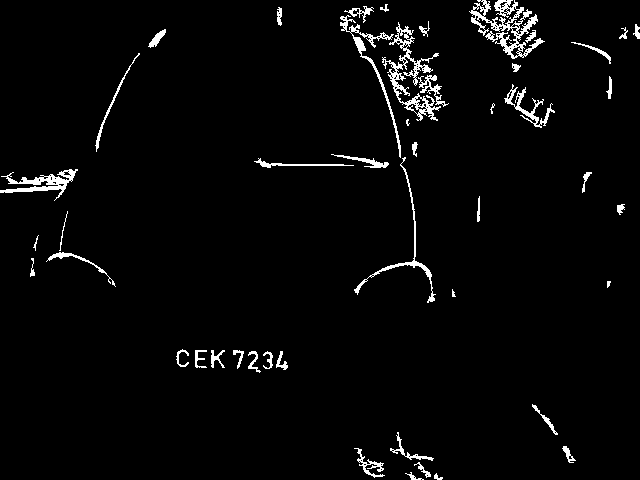
\includegraphics[scale=0.5]{img_relatorio/step2.png}
		\caption{Passo 3 - Eliminação de elementos finos}\label{step2}
		\end{center}
	\end{figure}
\newpage

\subsubsection{Passo 4 - Junção de dígitos da placa}
	É feita uma junção dos dígitos da placa para tornar possível a eliminação de partes da imagem que são menores que a união dos dígitos mas maiores que cada dígito individualmente e de partes maiores que a placa como um todo. O resultado pode ser visto na figura~\ref{step3}.
	\begin{figure}[!h]
		\begin{center}
		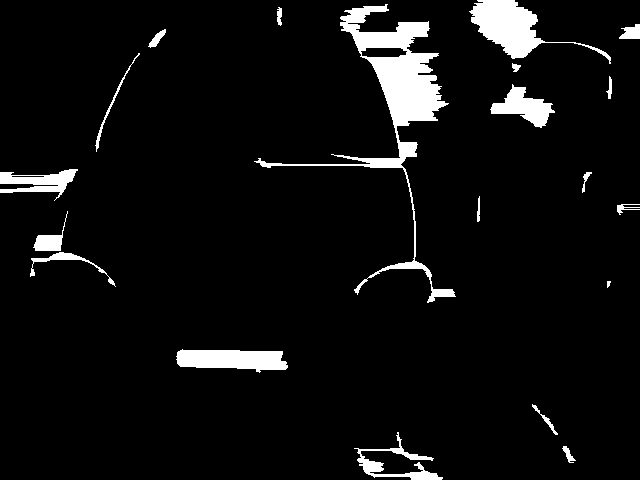
\includegraphics[scale=0.5]{img_relatorio/step3.png}
		\caption{Passo 4 - Junção de dígitos da placa}\label{step3}
		\end{center}
	\end{figure}
\newpage

\subsubsection{Passo 5 - Eliminação de elementos mais largos que a placa}
	Esta operação é um filtro conexo que elimina componentes que contenham um quadrado de tamanho $151\times1$, ou seja, componentes mais largos que uma placa. O resultado pode ser visto na figura~\ref{step4}.
	\begin{figure}[!h]
		\begin{center}
		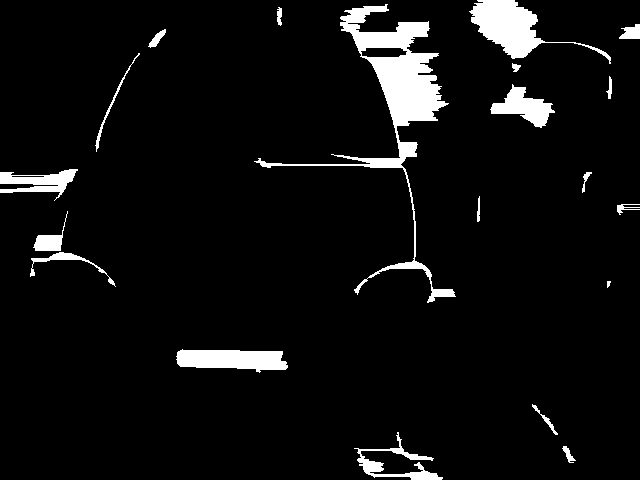
\includegraphics[scale=0.5]{img_relatorio/step4.png}
		\caption{Passo 5 - Eliminação de elementos mais largos que a placa}\label{step4}
		\end{center}
	\end{figure}
\newpage

\subsubsection{Passo 6 - Realce de elementos com tamanho similar ao da placa}
	Esta operação é um filtro conexo que mantém componentes que contenham um quadrado de tamanho $91\times45$, ou seja, componentes que possuam um tamanho maior que um retângulo que está contido na placa com "pouca folga". Esta operação mantém a placa e elimina toda parte da imagem que não pode conter uma placa. O resultado pode ser visto na figura~\ref{step5}.
	\begin{figure}[!h]
		\begin{center}
		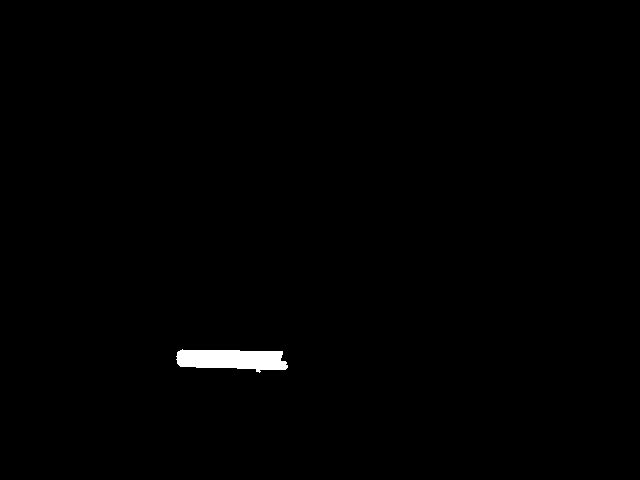
\includegraphics[scale=0.5]{img_relatorio/step5.png}
		\caption{Passo 6 - Realce de elementos com tamanho similar ao da placa}\label{step5}
		\end{center}
	\end{figure}
\newpage

\subsubsection{Passo 7 - Eliminação de elementos mais altos que a placa}
	Esta operação é um filtro conexo que elimina componentes mais altos que  51 pixels, ou seja, componentes mais altos que uma placa de carro. O resultado pode ser visto na figura~\ref{step6}.
	\begin{figure}[!h]
		\begin{center}
		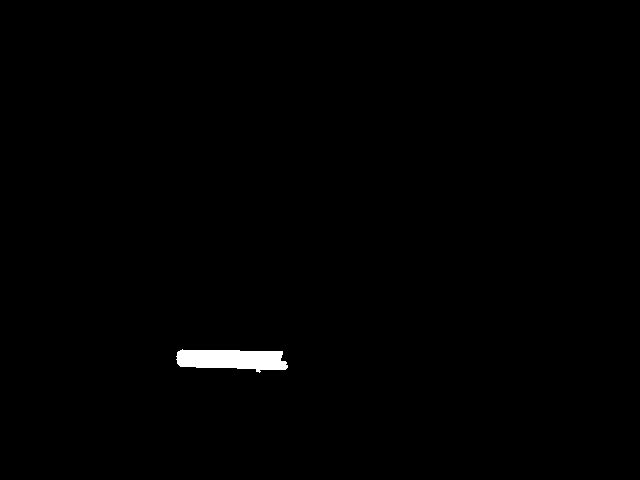
\includegraphics[scale=0.5]{img_relatorio/step6.png}
		\caption{Passo 7 - Eliminação de elementos mais altos que a placa}\label{step6}
		\end{center}
	\end{figure}
\newpage

\subsubsection{Passo 8 - Determinação dos marcadores finais}
	O marcador da placa é obtido dilatando o resultado do Passo 7 por um quadrado $11\times11$. O marcador de fundo é obtido dilatando o marcador da placa por um quadrado de tamanho $31\times31$ e visa obter uma borda exterior à placa. O resultado pode ser visto na figura~\ref{step7}.
	\begin{figure}[!h]
		\begin{center}
		
\includegraphics[scale=0.5]{img_relatorio/step7-markers.png}
		\caption{Passo 8 - Determinação dos marcadores finais}\label{step7}
		\end{center}
	\end{figure}
\newpage


\subsection{Segmentação utilizando Watershed}

O marcador de fundo é obtido fazendo-se uma dilatação do marcador da placa do  carro por um elemento estruturante tamanho $10\times10$. 

O algoritmo Watershed é aplicado utilizando como entrada a imagem original em níveis de cinza e os marcadores obtidos anteriormente e retorna o resultado final da segmentação, que pode ser na figura~\ref{final}.

\begin{figure}[!h]
	\begin{center}
	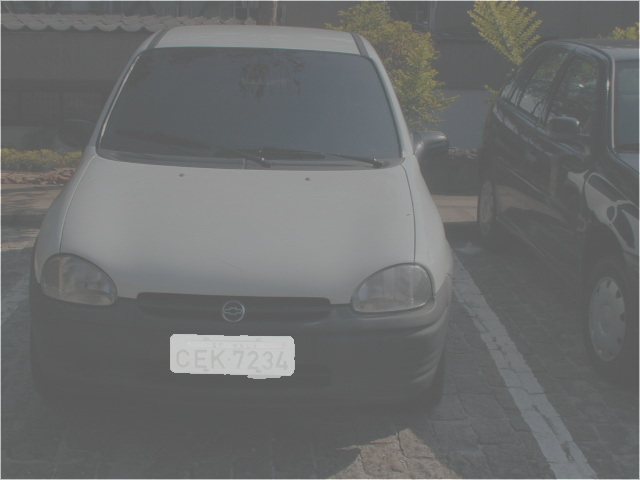
\includegraphics[scale=0.5]{img_relatorio/step8-final.png}
	\caption{Resultado final}\label{final}
	\end{center}
\end{figure}

\section{Resultados}

Os resultados das segmentações podem ser encontrados na pasta results. A única imagem em que não foi possivel obter o marcador de placa foi a {\em cts9360.png}, pois os elementos estruturantes usados não são adequados para o tamanho da placa nesta imagem, que é menor que as placas presentes em outras imagens.

Em geral as segmentações apresentaram alguma invasão tanto do fundo para a placa quanto da placa para o fundo, porém considerei os resultados obtidos bons por ter conseguido realçar em todas as segmentações os dígitos da placa, que são a principal informação contida nesta parte da imagem.

\end{document}
